\documentclass[a4paper, 11pt]{article}
\usepackage[titles]{tocloft}
\usepackage[utf8]{inputenc}
\usepackage{natbib} % eksempel til sitering: \cite{bass2003software}. referanser legges i ref.bib. Etter å ha oppdatert ref.bib må bibtex progArkDelivery1 kommando kjøres. 
\usepackage{hyperref}
\usepackage[pdftex]{graphicx}

%\newcommand{\HRule}{\rule{\linewidth}{0.3mm}}
\newcommand{\HRule}{\rule{\linewidth}{0.5mm}}

\title{\textbf{Action Hero Defense}\\\HRule\\Architectural Description\\ Group 23}
\author{\and Håvard Geithus
	\and  Sondre Løberg Sæter 
	\and Nicolai Meltveit 
	\and Hallvard Andreas Eriksen 
	\and  Håkon Drolsum Røkenes}
\date{\today}

\begin{document}

%\maketitle
\begin{titlepage}
\begin{center}

\vspace{10 mm}
{ \huge\bfseries Warcraft TD}\\[0.4cm]
Architectural Description\\
Group 23
\begin{figure}[h]
	\center
	
\includegraphics[scale=2]{images/peons}
\end{figure}

\vfill
\begin{minipage}{0.4\textwidth}
\begin{flushleft} \large
\emph{Authors:}\\
Håvard Geithus\\ 
Sondre Løberg Sæter\\ 
Nicolai Meltveit\\
Hallvard Andreas Eriksen\\
Håkon Drolsum Røkenes\\
\end{flushleft}
\end{minipage}
\begin{minipage}{0.4\textwidth}
\begin{flushright} \large
\emph{COTS:} Android-SDK \vspace{5 mm}

\emph{Quality Attributes:} \\

Modifiability\\ Testability\\ Usability
\end{flushright}
\end{minipage}
\vspace{10 mm}







%\vfill

% Bottom of the page
{\large \today}



\end{center}
\end{titlepage}



\tableofcontents
\clearpage

\section{Introduction}
This report will give an overview over the chosen architectures of the Action Hero Defense game, developed as a part of the TDT4240 course assignment.
We will focus on the reasons behind our choices of architecture, in addition to discussing how the chosen architecture conforms to the quality requirements which are set. Primarily the modifiability and testability quality requirements.

In the first section of this report, we will give an introduction on the architectural drivers of the game. This section will describe how the both the functional and quality requirements influence our choice of architecture. 

The next section, the architectural views, will offer a description of the architecture from different perspectives, or \emph{views}. Here we focus on two perspectives which we feel is most relevant for our project; the logical and the development view.

The Tactics-section will focus on the various techniques and methods we will employ to obtain the desired quality requirements, such as the modifiability 


Finally, we will discuss the design and architectural patterns we wish to implement in our system. We have decided on the Model-View-Controller architectural pattern and we will discuss how this pattern fits in to our selected quality requirements.


\section{Architectural Drivers}
\label{drivers} The architectural drivers are the combination of functional, quality, business and technical requirements which shape the architecture of the system \cite{bass2003software}.These are contributing factors which help decide on the architectural tactics for the system.  
In order to determine the drivers, one need to first identify the business goals of the system, then transform these goals into quality scenarios or use cases. 

Architectural decisions mainly focus on avoiding unnecessary complexity. The drivers are based on the use cases which will cause the highest complexity, while being of high importance in order to achieve the business goals.

In this section we will give an overview of the architectural drivers in our application. We will describe the tactics using 4 aspects; functional requirements, quality attribute requirements, business constraints and technical constraints.

\subsection{Functional requirements}
The following list contains the most important functional requirements that will shape the architecture of the system. The identification of each requirement is that from the requirements document\cite{reqdoc}.

\begin{itemize}
        \item \textbf{FR.1} Stop mobs using towers.
        \item \textbf{FR.3} Next wave after a wave finishes.
        \item \textbf{FR.4} Increasing mob strength.
        \item \textbf{FR.5} Earning gold to build new towers.
        \item \textbf{FR.6} Winning the game.
        \item \textbf{FR.11} Menu for building towers.
\end{itemize}

\subsection{Quality attributes}
Listed are the most important quality attributes for the architectural drivers. We will also here refer to the requirements described in the requirements document.

\subsubsection{Modifiability}
\begin{itemize}
        \item Add, remove and changing towers and their properties (QR.1 through QR.4)
        \item Easy to make new maps (QR.5).
\end{itemize}

\subsubsection{Testability}
\begin{itemize}
        \item Easy to access component state (QR.6)
        \item Log relevant information (QR.7)
\end{itemize}

\subsection{Business constraints}
\begin{itemize}
        \item Important for the application not to require uneccesary and unnatural manifest permissions.\footnote{http://developer.android.com/reference/android/Manifest.permission.html} For instance contact information on the phone.
        \item Use of software components under the GNU General Public License version 2 or later. Our system will have to released under this license. 
\end{itemize}

\subsection{Technical constraints}
\begin{itemize}
        \item None.
\end{itemize}



\section{Stakeholders}
\label{stakeholders}

Course staff - the concerns of the course staff would be how easy it is to
compile-and-run the final product, and how good the documentation of the code
is. These are concerns for them because they will evaluate our product according
to these criteria.
\newline
\newline
Android users - this stakeholder is an android user who wants to try
to play the game. One of the concerns for this stakeholder is how easy the game is to run and
play. This means that the instructions on how to play the game should be easily
available and easy to understand. The stakeholder is also concerned with how good the usability for the game is. That is, how easy the game is to get familiar with and the sense of control it provides.
\newline
\newline
Programmers - the programmers concerns are mainly with the implementation of the system. They want the architecture to be in such a way that further implementation and improvement is as easy to perform as possible. This can be achieved by using patterns in the implementation. Good documentation of the code is also a valid concern of the programmers.
\newline
\newline
Testers - good testability is the main concern for the testers. They want the system to be as easy to test as possible, to ensure that all features can be checked properly. Good testability will result in less work for the testers, and thus, lower costs.
\section{Architectural views}
In this section we will give a description of the diagrams created as a representation of our selected architectural viewpoints. As mentioned in the previous section we focus on the logical and development viewpoints, and these will be represented with a class diagram and a package diagram, respectively -- to be found in the appendix of this report.

\subsection{Logical View}

The logical view is illustrated by the class diagram in figure \ref{fig:classdiagram}. This diagram tries to illustrate the logic between the most essential classes in the system, and the relationships between them. 

The Game and TowerDefenseState instances are constructed in the PlayActivity. The Game object holds a stack of game states, and the TowerDefenseState is pushed onto this stack. It is the only state of the game. There is also a MenuActivity (not shown in the class diagram for simplicity), which is a simple menu showed in the GUI, with buttons to initialize the game. When the game is initialized, the control is passed over to the PlayActivity.

The system is focused around various classes with "controller" as postfix, initially for convention in regards to the MVC-pattern. 
These classes have different levels of responsibility for handling input and initiating response for the inputs.

The TowerDefenseState-class extends the class State (from the Sheep-framework) and behaves as the top controller of the system. It's responsibilities include invoking the draw and update methods on it's super-object (State), as well as all the subcomponents displayed on the screen. The components which contains draw and update methods are, in particular, the Sprite-objects (towers and enemies).

The GameController-class is, as it's name implies, responsible for handling the flow of the game. It decides when a new wave of enemies should be spawn, as well as when towers should shoot at enemies.  

WaveController handles the waves of enemies, through Wave-objects -- which contains information of a particular wave. The WaveController decides which wave should be spawned next.

SpriteFactory is responsible for producing Sprites-objects, both EnemySprite and TowerSprite. A TowerSprite needs a model for it to be instantiated. The model decides the uniqe properties of a particular tower. 


\subsection{Development View}
Figure \ref{fig:packagediagram} illustrates a package diagram showing the development view of the system. The diagram illustrates the most essential packages and their components.

As mentioned in the previous section, some of the naming conventions relates to the MVC-pattern and this is also a case in regards to the package-names. The MVC-pattern is not fully implemented in the system, something which we will elaborate more in later sections, however it seemed natural with this naming convention nevertheless.

The controller package could also be named the "core" package in system. Components in this packages are responsible for initiating and controlling the flow of the game. Included in these components are action- and eventlisteners, registering input and events occuring during gameplay.

The view package includes the sprite-components -- which in turn contains functionality for drawing dynamic objects on the screen. In addition, a component for creating such sprites is also included in this package.

We try to seperate business logic into the model-package. For instance, the path of an enemy sprite is computed in the EnemyPath-class in the "model.game"-package. 

The COTS libraries, Android SDK and the Sheep framework, are also illustrated in the diagram, showing the dependencies drawn from these.

It should be worth mentioning that we try to keep in mind the Single-responsibility principle, in which a class should have only one responsibility. In turn, packages should also have one main area of responsibility. However, in some cases this principle was not entirely maintained as is the case in the controller-package. The area of responsibility in this package includes both the controlling of inputs and the actual gameflow. 

It should also be noted that when stating that a component is the "heart" of a system, we are in danger of creating so-called "God"-classes which has too much responsibility. It can be argued that our architecture is in danger of this problem when declaring the "controller"-package as the core module of the system. However, responsibility within this package is delegated into several sub-components, with no component having too much responsibility. This can perhaps be argued on the basis of lines of code, in which no class in the package has more than 400 lines.



\subsection{Consistency among views}

The logical view presents the individual classes of the system, and the relationship between them. In the development view, we present a more overall view of the architecture by including packages.

The consistency between the views is maintained by including the classes in the logical view as compononents in a package, in the development view. Relationships between classes in the logical view is also maintained by having the same relationships between the relevant packages in the development view. 

\section{Tactics}
\label{tactics}
To achieve the desired quality attributes one can apply tactics. Tactics are design options that can be taken to achieve qualities. In this chapter we will present tactics for all attributes, including the ones we have our main focus on, which are modifiability, testability and usability. 

\subsection{Modifiability}
The modifiability attribute concerns how easy it is to make changes to the system. The main concern is how much a change is going to cost in terms of extra work needed to be done to make this change functional. A change scenario consists of the following factors:

\begin{itemize}

	\item Source - the person that wants to make the change
	\item Stimulus - the change the source wants to perform
	\item Artifact - what the source wants to change
	\item Environment - when this change shall be performed
	\item Response - what response
	\item Response measure - how much this change will cost, in regards to money and elements affected
\end{itemize}

After this has been specified one has to design, implement, test and deploy the change. In regards to this the extent of modifiability will determine how much this operation will cost. By employing the following tactics one can increase the modifiability: 

\begin{itemize}
	\item Localizing changes - divide the responsibilities to modules during design so changes will be limited to that module
        \begin{itemize}
	\item Generalize the module - make the module able to provide more functions based on different inputs by making it more generalized. This can for example be achieved by using the Abstract Factory pattern
	\item Minimize dependencies - if modules are less dependent of each other, they will not be as affected by changes
	\end{itemize}
	\item Platform independent - make the game able to run on several different versions of Android
	\item Single responsibility principle - make one module responsible for one function. If it is responsible for more than one function, divide the module into several classes, with one responsibility for each class
	\item Clean code - write the implementation in clean code, which is easy to understand and unambiguous
	\item Documentation - provide good documentation and commenting of the code to ease the job for other programmers
	
	\item Prevention of ripple effects - prevent changes on one module from affecting the entire system.
        \begin{itemize}
	\item Hide information - use encapsulation to keep information in different modules invisible to each other
	\item Restrict communication paths - use of encapsulation will help in restricting communication paths, resulting in less interaction between the modules in cases of errors
        \end{itemize}
\end{itemize}


\subsection{Testability}
The testability attribute concerns how easy the system is to test and how much the testing process will cost. Testing is usually a big resource drain, but at the same time such a crucial part of the system creation process that it cannot be neglected. The key is to make testing less expensive by ensuring good testability for the system. The goal of the testability tactics is to make a system testable, by making it possible to control the internal states and inputs of the components and observe the outputs \cite{bass2003software}. Tactics one can employ to achieve good testability are: 

\begin{itemize}
	\item Input/Output handling
        \begin{itemize}
	\item Separate the different types of components - keep components such as logic, view, models separate which will make writing tests for specific parts much easier. Separation of interfaces from the system will make testing by code insertion possible without affecting the whole system.
	\item Keeping classes at low complexity - smaller classes will also make the test classes smaller and easier to write. Makes testing of specific parts of the system easy.
	\item Console output - write outputs to the console to check if modules give the expected results.
	\end{itemize}
    
	\item Internal monitoring
        \begin{itemize}	
        \item Employ logging - makes it possible to observe the inputs and outputs of components so one can check after a test if it has been performed as expected.
        \end{itemize}
	\item Use COTS - use testing COTS(Commercial, Off-The-Shelf).
\end{itemize}


\subsection{Usability}
Usability describes how easy and user friendly the system is the for the end user. Any system which has an end-user as a stakeholder should take usability into consideration. The importance of usability depends on how important the end-user is for the system. Usability tactics can be divided into two types, to support to categories of users. The first category is called runtime and includes those that support the user during system execution. The second category is design-time and supports the interface developers.\cite{bass2003software} For runtime the follow tactics are provided:

\begin{itemize}
	\item Abstract errors from the user - abstract error messages from the user interface in such a way that the user never knows if anything went wrong, in cases the error is fixed without any problems.
	\item Maintain models - the application should maintain models of the task, the user and the system, to make handling events easier by keeping the interacting parts separate.
\end{itemize}

Design-time tactics are:

\begin{itemize}
	\item Separate the user interface from the rest of the application - one can apply an architectural pattern such as MVC to separate the GUI modules from the logic. This will make changes to the user interface easier to implement.
\end{itemize}

\subsection{Availability}
Availability is concerned with how accessible the system is at all times that is, how big the consequences of a system failure is. It is important to distinguish between faults and failures. A fault may become a failure if not corrected, and a failure is observable by the system's user and a fault is not\cite{bass2003software}. The key tactics to ensuring good availability are: 

\begin{itemize}
	\item Fault detection - faults in the system are detected and reported to the other parts.
        \begin{itemize}
	\item Ping/echo - the system can ping a process to see if it is alive and functional.
	\item Throw exceptions - the system can detect errors by having failing processes that fail call exceptions.
	\end{itemize}
	\item Fault recovery - the system should be able to recover as fast/good as possible after a fault has happened.
        \begin{itemize}
	\item Checkpoint/rollback - the system should be able to enter a previous consistent state if a fault should occur.
	\end{itemize}
	\item Fault prevention - faults should be prevented, and their effects should be isolated from the rest of the system.
\end{itemize}


\subsection{Performance}
Performance is concerned with how efficient the system is at resource handling and event processing. The key tactics to improve performance is to establish better use of the systems resources. Tactics included are:

\begin{itemize}
	\item Resource management - used to ensure concurrency, run separate threads.
	\item Resource arbitration - used to provide scheduling of resources according to priority assignment.
	\item Resource demand - used to reduce the resources needed and number of processed events.
\end{itemize}

\subsection{Security}
Security is concerned with how resilient the system is towards unauthorized usage while still being able to provide its users with the intended services. Key tactics to ensure good security are:

\begin{itemize}
	\item Intrusion detection - detection of intrusion or attempts of intrusion in the system.
	\item System recovery - the system should be able to recover after an attack has been made or prevented.
	\item Ability to resist attacks - the system should be able to withstand attacks. 
\end{itemize}

A secure system is characterized by the following qualities:

\begin{itemize}
	\item Nonrepudiation - transaction cannot be denied by parties to it
	\item Confidentiality - data and services are protected against attacks
	\item Integrity - data and services are delivered as intended
	\item Assurance - correct parties of a transaction
	\item Availability - available for legitimate use
	\item Auditing - tracks activities in order to reconstruct them
\end{itemize}

\section{Patterns}
This section will be a discussion on the architectural and design patterns to be employed in the Action Hero Defense game. There will be a presentation of the patterns to be used, explaining why the particular pattern was chosen and how we plan to implement it.

\subsection{Architectural pattern}
\subsubsection{MVC}
For the overall design of our application we have chosen the \textbf{Model-View-Controller} (MVC) pattern, which focuses on separating the domain, or application, logic of an application, from the user interface. It consists of tree different structures\cite{wiki:mvc}:
\begin{itemize}
\item \emph{Model} - responsible for managing the behavior of the system. This is where the main functionality and data management of the system should reside.
\item \emph{View} - typically the user interface of the system. Responsible only for drawing or displaying information on screen. The data which is supposed to be shown, is generated and managed in the model.
\item \emph{Controller} - manages input from the user in addition to what should be the following response from the system. An input may instantiate an action for either the model and/or view. 
\end{itemize}

 
A MVC-pattern provides several benefits. In our case the separation of domain logic and user interface provides a solid foundation for supporting the main quality attributes of our system; modifiability and testability. 

If we consider a model responsible for the core functionality of a system, the ability to add a new feature would mainly be concerned with the model of the system, limiting modification to only one module. This way we ensure a loose coupling between the different modules of the system, and thus making it easier to modify a single part of the system. In addition, the MVC-pattern could also help prevent ripple effects which can occur when a module is changed. A change in the user interface would not change anything in the model, and vice versa, a change in one of the methods of the models would not interfere with the user interface, as long as the method still returns the same type of value. 


The testability-aspect also benefits greatly of the isolation of domain logic, especially when considering unit testing of a system. A unit-test should not have to be concerned with what happens in the user interface, it should only focus on the behavior of the domain logic. What happens when a user press a button at the user interface should not be the unit tests responsibility. Tests concerning dependency and communication between modules would be more of an integration test's responsibility. 


With unit testing, the model will again be the main focus point. Unit test can be applied to only the model of the system. If a test would require user input to test a certain function, the tests-classes should be responsible for generating mock values to simulate user input. In this way, the functionality can easily be tested in isolation and with no dependency of the user interface. We should however assume that some form of design patterns and principles within the model are being practiced.


For our tower defense game, the MVC-pattern will be responsible for defining the architecture. The View of the software will be responsible for drawing and animation of the sprites and images on screen, whereas the controller will naturally be responsible for taking user input, and communicating this input to the view and model. The model will be responsible for monitoring and managing the status of both the game, the player and the enemies. The status of an enemy will for instance be changed when a cannonball hits the enemy, and the object, located in the model section,  responsible for monitoring the enemy's health status will be invoked. 

A (preliminary) concept of how the MVC-model should work in practice is as follows: an event, say a tower shoots at an enemy, will be first processed by the view which animates the particular event. As the cannonball-sprite collides with the enemy-sprite, a collision-event should occur. The collision detection would here be part of the controller, which then proceeds to invoke the model which in turn updates the enemy (and game) status. 
\subsection{Design Pattern}
\subsubsection{Singleton Pattern}
When implementing the Singleton design pattern, one restricts the instantiation of a class to one object. The purpose of this is to allow visibility for a class in the entire system. While the singleton pattern does not increase the modifiability, which is the main quality attribute the system is supposed to incorporate, it is important to keep track of the state of the system. The singleton pattern introduces many dangers, such as mutual dependencies, which usually increase the complexity of the system. It is important to maintain proper synchronization in a multi-threaded environment, with the introduction of Singleton pattern (global variables).

Singleton classes have few differences from a static class, but the main difference is that a Singleton class allows lazy initialization. Lazy evaluation is an evaluation strategy which allows a class to only initialize if needed. That way, resources may be saved. Resource usage is usually something which affects the performance quality attribute, which is not the main focus for this project. That aside, performance is still a factor which should not be ignored. \cite{wiki:singleton}

The different quality attributes affect each other, and some affect each other in negative way. In the case of Singleton pattern, which could be looked at a pattern increasing performance in many cases, it reduces modifiability, but increases performance.  

\subsubsection{Abstract factory}

\begin{figure}[h]
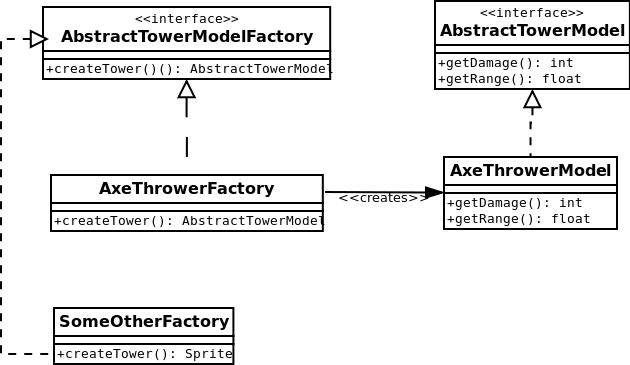
\includegraphics[width=1\linewidth]{images/abstractFactory.png}
\caption{Class diagram of the abstract factory pattern}
%\label{fig:absfac}
\end{figure}

The abstract factory pattern concerns the creation of objects. The main idea is that it provides an interface for the creation of related objects, without specifying the concrete classes. A normal way of incorporating this pattern would be to create a concrete implementation of an abstract factory, which creates concrete classes, and letting the client code be unaware of the concrete implementation, all it needs is an object implementing the abstract factory. \cite{wiki:abfac}  


In our case, the abstract factory would be useful when creating similar objects which will be in frequent use. An example of this is the sprites which will be displayed on the screen, for instance generating enemies. The enemy-objects could be similar, however with some unique properties. In this context an abstract enemy factory would seem like a good design solution. A diagram illustrating the concept is shown below:



We should here assume that we have a Sprite interface, an interface which we use to display all of the graphical objects on the screen. Relating it to the MVC, we could also assume that such a Sprite have a corresponding model-object, where we also could employ the abstract factory design pattern. 

As it stands, these are the main patterns we will focus on implementing to our Android game. 

\begin{verbatim}Øvrig TODO:
Views:
· A Process View is necessary.
· Enough details like important methods and attributes should be included in the logic view to make a complete picture of the software.
Consistency Among Views: Missing!
Rationale: Missing.
Issues: Missing
\end{verbatim}

\bibliographystyle{plain}
\bibliography{ref}
\end{document}
